\documentclass{report} 

\usepackage{amsmath} % \usepackage is a command that allows you to add functionality to your LaTeX code
\usepackage{graphfig, subfig}


\usepackage[Glenn]{fncychap}
\title{Storytelling} % Sets article title
\author{Emmanuele Virginio Coppola, Muriel Rossi, Alessandro Marigliano} % Sets authors name

\begin{document} % All begin commands must be paired with an end command somewhere 
    \maketitle % creates title using information in preamble (title, author, date)  $\downarrow$   \date{\today} % Sets date for date compiled

    \tableofcontents
    \chapter{Introduzione} % creates a chapter
    
    La pubblicità invasiva si rivela essere sempre maggiormente un problema asfissiante all'interno del mondo dei socialnetwork. Nonostante siano state sviluppate diverse tecniche
    allo scopo di domare questa piaga, alcune inserzioni riescono tuttavia a sfuggirne, intasando interfacce dedicate all'informazione ed 
    all'intrattenimento, che subiscono così una svalutazione, venendo "soffocate".
    

    \textbf{Legge di Reed: il valore di una rete sociale è direttamente proporzionale ad una funzione esponenziale in N:}
    \begin{equation} % Creates an equation environment and is compiled as math
        V=a*N+b*N^2 + c*2^n
    \end{equation}
    

    La legge sopra citata, descrive come il valore di una rete, formata da interazioni ed intrecci, cresca esponenzialmente con la dimensione di quest'ultima. (1.1).
    In particolare, nel caso di Internet, si osserva come il suo valore tenda a crescere in modo esponenziale se associato a gruppi con interessi
     comuni, che condividono idee, interessi ed obiettivi.
    Da questo se ne deduce come invece, avvisi pubblicitari, spam ed altra "informazione spazzatura", possano far decadere il valore di una rete.
    
    Questo progetto si prefigge lo scopo di manutenere una piattaforma libera dal bombardamento pubblicitario e dare modo all'utenza di potersi esprimere liberamente
    all'interno di questa, distaccandosi dall'ansia e dalla continua distrazione provocata dal chiasso delle inserzioni.
    \chapter{Descrizione dell'agente}
    Allo scopo di realizzare questo progetto, è stato introdotto un agente intelligente, sarà lui ad occuparsi della supervisione della piattaforma, indagando fra i 
    commenti relativi alle varie pubblicazioni.
    \section{Obiettivi}
    L'obiettivo dell'agente sarà quello di effettuare un'analisi giornaliera dei commenti relativi ad ogni pubblicazione effettuata dagli utenti della piattaforma.
    Il testo dei vari commenti verrà preso in analisi e, dopo essere stato adeguatamente "pulito", verrà sottoposto all'agente, che sarà in grado di riconoscere se il 
    testo è conforme alle norme della piattaforma (ovvero se non è sospettato come spam). \newline
    In caso negativo, l'autore del commento verrà segnalato alla piattaforma, che provvederà ad eliminarlo da quest'ultima, assieme a tutto il materiale da lui pubblicato.

    \section{Specifiche PEAS}
    Le specifiche PEAS rappresentano diverse proprietà tramite cui è possibile descrivere l'agente. \newline

    \begin{itemize}
        \item 
        {\bfseries P = Performance.} 
        L'agente verrà valutato in base alla percentuale di commenti spam categorizzati correttamente.
        \item 
        {\bfseries E = Environment.} L'agente nel caso in questione lavorerà su query di commenti relativi ai post pubblicati sul Social Network, 
        navigando fra i commenti degli utenti.\newline
        Nello specifico l'ambiente sarà:
            \begin{itemize}
                \item {\bfseries Completamente Osservabile}, in ogni momento l'agente ha completa conoscenza
                dell'ambiente in cui lavora, ovvero la collezione di commenti;
                \item {\bfseries Deterministico}, l'ambiente verrà modificato in base alla decisione dell'agente, 
                ovvero verranno rimossi gli utenti che l'agente deciderà di segnalare;
                \item {\bfseries Episodico}, l'agente viene attivato ad intervalli temporali di 24h. La scelta che
                compirà l'agente in un singolo episodio dipenderà dall'episodio stesso;
                \item {\bfseries Statico}, mentre analizza la query di commenti, l'ambiente rimane invariato;
                \item {\bfseries Discreto}, l'ambiente infatti fornisce un insieme di parole finite per ogni commento. L'agente
                dovrà decidere orientandosi fra queste ed avrà azioni limitate (segnalare l'utente o non farlo); 
                \item {\bfseries Singolo}, l'agente che opererà sarà singolo.
            \end{itemize}
          
        \item 
        {\bfseries A = Actuators.} L'agente potrà effettuare il suo giudizio stilando una lista di email relative ai proprietari dei commenti che sono stati sospetatti di spam.
        \item 
        {\bfseries S = Sensors.} Il modo in cui l'agente riceverà gli input percettivi sarà tramite il dataset di commenti.I sensori attraverso cui riceve gli input percettivi.


        
      \end{itemize}
    

    

                        


   
    \chapter{Raccolta, analisi e preprocessing dei dati}
    \section{Scelta del dataset}
    \section{Pulizia del dataset}
    \section{Bilanciamento del dataset}
    Il dataset è bilanciato.
    \begin{figure}
        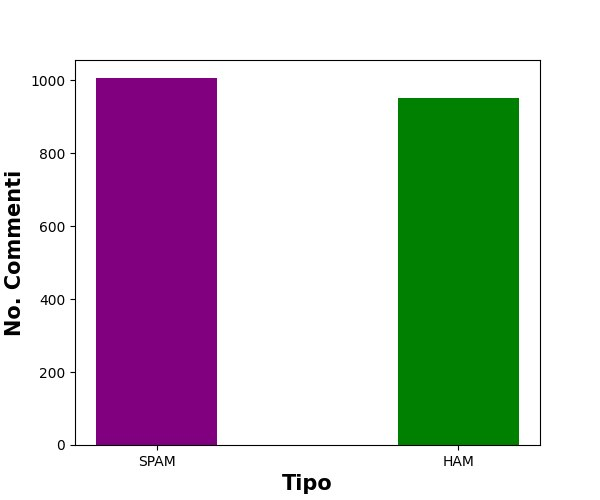
\includegraphics[width=0.7\columnwidth]{immagini/datasetMergiato.jpg}
    \end{figure}
    \chapter{Creazione agente}
    Dopo aver definito gli obiettivi dell'agente, le sue specifiche, l'ambiente in cui avrebbe lavorato, ed il suo dataset, si è deciso come andava effettivamente costruito l'agente.
    L'agente dovrà stimare se un commento è un avviso pubblicitario o meno con il solo aiuto delle parole presenti nel commento. Inizialmente è stato sottoposto all'agente 
    un dataset di commenti, ognuno dei quali era contrassegnato da un target "SI", se lo specifico commento era spam, o contrassegnato da target "NO" se il commento era ham.
    E' quindi stata creata una tabella dove venivano individuate, per ciascun commento,
    la frequenza con la quale alcune parole ricorrevano. In questo caso ci è venuto in aiuto l'algoritmo {\bfseries Naive Bayes}:
    \newline
    \begin{equation}\label{bho}
       % { p(B|A)  p(A)\over p(B)}
    \end{equation}
    \newline
    che, nel nostro caso, si traduce in:
    \newline
    \begin{equation}\label{bho2}
        p(spam|commento) = { p(commento|spam)  p(spam)\over p(commento)}
    \end{equation}
    \newline
    ovvero, la probabilità che un commento sia spam, è uguale alla probabilità che le parole del commento compaiano in un commento spam, dato che è spam, per la probabilità 
    che il commento sia spam, diviso la probabilità che queste parole compaiano nel commento.



\end{document}